\documentclass[a4paper, 11pt, ngerman, fleqn]{article}
\usepackage[utf8]{inputenc}
\usepackage[ngerman, english]{babel}
\usepackage{coordsys,logsys,color}
\usepackage{hyperref}
\usepackage{texdraw}
\usepackage{fancyhdr}
\usepackage{graphicx}
\input{txdtools}

\NeedsTeXFormat{LaTeX2e}
\ProvidesPackage{hyperref}
\definecolor{darkblue}{rgb}{0,0,.6}
\hypersetup{pdftex=false, colorlinks=true, breaklinks=true, linkcolor=black, menucolor=darkblue, urlcolor=darkblue, citecolor=darkblue}

\pagestyle{fancy}

%\renewcommand{\familydefault}{cmss}

\definecolor{fgcgray}{rgb}{0.4, 0.4, 0.4}
\definecolor{warning}{rgb}{0.9, 0.1, 0.0}
\definecolor{bgctitle}{rgb}{0.5, 0.5, 0.5}
\definecolor{fgctitle}{rgb}{0.95, 0.95, 0.95}
\newcommand{\titlefont}[1]{\textcolor{fgctitle}{\fontfamily{cmss}\fontseries{bx}\fontshape{n}\fontsize{20.48}{0pt} \selectfont #1}}
\newcommand{\inversetitlefont}[1]{\textcolor{bgctitle}{\fontfamily{cmss}\fontseries{bx}\fontshape{n}\fontsize{20.48}{0pt} \selectfont #1}}

\addtolength{\oddsidemargin}{-1.0cm}
\addtolength{\evensidemargin}{-1.0cm}
\addtolength{\headwidth}{2.0cm}
\addtolength{\textwidth}{2.0cm}

%\setlength{\parindent}{0cm}

\renewcommand{\labelitemi}{$\circ$}
\renewcommand{\labelitemii}{$\diamond$}

\newcommand{\spaceline}[1][8pt]{\vskip #1}
\newcommand{\comment}[1]{\spaceline[5pt] \textcolor{fgcgray}{\scriptsize #1} \spaceline[15pt]}
\newcommand{\attrname}[1]{\textcolor{fgcgray}{\scriptsize #1}}


\makeatletter

\newcommand*{\project}[1]{\gdef\@project{#1}}
\newcommand*{\version}[1]{\gdef\@version{#1}}
\newcommand*{\home}[1]{\gdef\@home{#1}}
\newcommand*{\homeref}[1]{\gdef\@homeref{#1}}

\def\@maketitle{
  %\begin{titlepage}
  \begin{center}
    \colorbox{bgctitle}{
      \parbox{\textwidth}{
        \spaceline
        \centering{\titlefont{\@title}}
        \par
        \spaceline
      }
    }
    \colorbox{white}{
      \parbox{\textwidth}{
        \spaceline
        \centering{\inversetitlefont{\@project}}
        \par
        \spaceline
      }
    }
  \end{center}
  \spaceline[1.5em] {
    \begin{flushright}
    \begin{tabular}[t]{rl}
      \attrname{Project:} & \@project ~ \@version \\
      \attrname{Author:} & \@author \\
      \attrname{Last Change:} & \@date
    \end{tabular}
    \end{flushright}
    \par
  }
  \spaceline[5.5em]
  %\end{titlepage}
}

\setcounter{secnumdepth}{4}
\setcounter{tocdepth}{4}

\newcounter{subsubsubsection}[subsubsection]
\def\subsubsubsectionmark#1{}
\def\thesubsubsubsection{\thesubsubsection .\arabic{subsubsubsection}}
\def\subsubsubsection{\@startsection{subsubsubsection}{4}{\z@}{-3.25ex plus -1 ex minus -.2ex}{1.5ex plus .2ex}{\normalsize\bf}}
\def\l@subsubsubsection{\@dottedtocline{4}{4.8em}{4.2em}}

\makeatother

\everytexdraw{
  \drawdim cm \linewd 0.01
  \arrowheadtype t:T
  \arrowheadsize l:0.2 w:0.2
  \setgray 0.5
}

\newcommand{\xheight}{0.6}
\newcommand{\xlength}{0.6}
\newcommand{\yheighta}{1.0}
\newcommand{\yheightb}{0.8}
\newcommand{\yheightc}{0.6}
\newcommand{\yheightd}{0.5}
\newcommand{\yheighte}{0.4}
\newcommand{\yheightf}{0.35}

\newcommand{\xhline}{\rlvec({\xlength} 0)}
\newcommand{\xharrow}{\ravec(0.7 0)}
\newcommand{\xnext}{%\rlvec(0.05 0) \lpatt(0.04 0.04) \rlvec(0.15 0) \lpatt()
}

\newcommand{\xtext}[3][\xheight]{
  \bsegment
    \bsegment
      \setsegscale 0.5
      \textref h:L v:C  \htext({\xheight} -0.1){#3}
    \esegment
    \setsegscale 0.5 \lvec(0 #1)
    \setsegscale 1
    \rlvec(#2 0) \rlvec(0 -#1) \rlvec(-#2 0) \lvec(0 0)
    \savepos(#2 0)(*@x *@y)
  \esegment
  \move(*@x *@y)
}

\newcommand{\bxtext}[3][\xheight]{
  \setgray{0.1}
  \linewd{0.026}
  \xtext[\xheight]{#2}{#3}
  \linewd{0.01}
  \setgray{0.5}
}

\newcommand{\xstartpage}{\bxtext{2.1}{Startseite}}
\newcommand{\xmainpage}{\bxtext{2.3}{Hauptseite}}
\newcommand{\xusermenu}{\bxtext{2.9}{Benutzermenu}}
\newcommand{\xgamelist}{\bxtext{2.2}{Spieleliste}}
\newcommand{\xportfolio}{\bxtext{2.0}{Portfolio}}
\newcommand{\xaccount}{\xtext{3.8}{Kennung per \textsl{eMail}}}


\begin{document}
  \lhead{\sc{Virtual Reality for Sensor Data Analysis}}
%\cfoot{-~\thepage~-}
\title{Software Specification}
\project{Virtual Reality for Sensor Data Analysis}
\version{2.0}
\author{Gero Birkhölzer, Johannes Blank, Alexej Gluschkow, Fabian Klopfer, Lisa-Maria Mayer}
\maketitle
%\thispagestyle{empty}
%~
%\newpage
%\tableofconte \newpage
  \tableofcontents \newpage
  \section{Purpose}

The software project in the summer term 2017 at the University of Constance focuses on the development of apps for mobile devices. In the course of the project an Android app is being developed which allows the user to explore sensor data in virtual reality.

Especially, this Software Requirements document intends to describe the functionality and requirements of the app being developed. Furthermore, the internal structure of the app as well as some test cases are specified.

\subsection{Product Idea and Goal}

The general idea of the product is to allow the user to record data about their environment and later explore the data in a three-dimensional scene via virtual reality. Therefore, the developed product will consist of two parts:

Firstly, the app itself. It's main goal is to connect to an external sensor device via Bluetooth and to process and save the data collected by the sensor (referred to as ``app''). \\
In order to view the saved data, the second part consists of a web application where a virtual reality scene is generated and the stored data are visualized (referred to as ``web application''). 

These two parts will be connected in such a way that the user can open a browser with the according web application from within the app.



%The general goal of the app consists of two parts: \\
%First, the user shall be able to record data with a sensor connected to the user's smartphone via Bluetooth and save the data as a function of the respective location. \\
%As the second part, the gathered data shall be displayed in a 3D environment which the user can explore in Virtual Reality. By displaying the data in regard to the location where it was recorded, it can be expierienced like a three-dimensional function where the user can navigate using a joystick. \\
%If possible, it would be nice to be able to watch the graphs visualising the data change over a period of time. This would be like watching the data in a video while being able to navigate through the graph.


\subsection{Definitions}

\begin{description}
	\item[App] When the app itself is mentioned, we refer to the application running on the smartphone that, as stated above, handles the recording of data and invokes a web browser with the web application.
	\item[Web application] This term refers to the web site that can be invoked by the app, runs in a web browser, and provides the virtual reality display of the data gathered by the app.
	\item[Sensor (device)] When referring to the sensor, we're talking about the sensor device (more clearly spezified in section 2) containing several sensors. 
	\item[Data] With data we generally mean information that has been gathered by the sensor.
	\item[Virtual Reality (scene)] This term describes the three-dimensional world in which the data will be displayed. 
	
\end{description}


\subsubsection{Abbreviations}

\begin{description}
	\item[TI] Texas Instruments
	\item[VR] Virtual Reality
	\item[3D] three-dimensional
	\item[DB] Database
	\item[App] Application
	\item[BLE] Bluetooth Low Energy
\end{description}

\subsubsection{Glossary}

\begin{description}
	\item[Stereoscopic 3D] The impression of 3D is created by rendering different pictures for every eye of the viewer.
	\item[Virtual reality] By using a headset in which the smart phone can be integrated, the user can view the three-dimensional world in stereoscopic 3D and thereby experiences the feeling of being fully immerged in the scene.
	\item[Augmented reality] Displaying 3D objects in a real-world surrounding while providing an immersive experience like virtual reality.
	\item[Gyroscope sensor] Sensor for measuring orientation in space.
	\item[Web application] Web site that offers functionalities similar to those of ``normal'' desktop or mobile applications but runs in a web browser.
	\item[Service] From \href{https://developer.android.com/guide/components/services.html}{AndroidDoc}: ``A Service is an application component that can perform long-running operations in the background, and it does not provide a user interface''.
	\item[GUI] From \href{https://developer.android.com/guide/components/activities.html}{AndroidDoc}: ``They (Activities) serve as the entry point for a user's interaction with an app, and are also central to how a user navigates within an app (as with the Back button) or between apps (as with the Recents button)''.
\end{description}

\bigskip

\subsection{Mandatory Criteria}

\begin{description}
	\item[M1] The app shall use the Bluetooth adapter of the smartphone to connect to the sensor.
	\item[M2] The app shall track the position of the sensor with up to 10m tolerance.
	\item[M3] The app shall store the data retrieved from the sensor.
	\item[M4] The web appliaction shall display a virtual reality scene using the WebVR framework.
	\item[M5] The web application shall display the stored data within the virtual reality scene depending of their respective location.
	\item[M6] The virtual reality scene in M4 shall be explorable for the user by using an external controller.
	
\end{description}

\subsection{Desired Criteria}

\begin{description}
  \item[D1] The product could contain a visualization of the stored data in augmented reality.
  \item[D2] The virtual reality world could represent more than a single scene.
  \item[D3] The product could contain the functionality to view not only one set of data at a time but to gerenerate a time lapse of the data that can be experienced like an interactive video where the user can move around and change the camera perpective.
  \item[D4] The product could provide functionalities to interact with more than one sensor.
  \item[D5] The app could provide an advanced way to determine the location where the data are recorded in order to improve the display of the data.
\end{description}
 \newpage
  \section{Product Environment}



\subsection{Software}

\begin{itemize}
  \item Android (5.0 Lollipop or higher)
  \item Google Chrome (Version 58.0.3029.110 or higher) (referred to as ``browser'')
\end{itemize}

\subsection{Hardware}

\begin{itemize}
  \item Bluetooth-enabled Smartphone (referred to as ``smart phone'')
  \item TI SimpleLink SensorTag device (referred to as ``sensor'')
  \item Victorstar VRBox 2.0
  \item VR-Park Bluetooth Controller
\end{itemize}
 \newpage
  \section{Product Functions}

%\comment{functional Requirements}
In the following, the required functionalities of the product are stated.

\subsection{Features of the App}

The app itself provides functionalities to interact with the sensor (such as to connect and retrieve data), to handle the data (process and store them in a way the web apliccation can acces them) and to invoke the web application.

\subsubsection{General Features}

\begin{description}
  \item[F1.1] The app shall be able to connect to a sensor.
  \item[F1.2] The app shall be able to store information about the location where a set of data is recorded.
  \item[F1.3] The app shall provide a live data view of the sensor feedback in human readable form.
  \item[F1.4] The app shall be able to save the data transferred from a connected sensor.
  \item[F1.5] The app shall be able to invoke the web application inside a browser.
  \item[F1.6] The app shall be able to link all recorded data to the location where they were recorded.
  \item[F1.7] The app shall shall save every set of data together with the respective location.
\end{description}

\subsubsection{Settings}

\begin{description}
      \item[F2.1] The app shall be able to show information about the sensor (such as settings and state).
      \item[F2.2] The app shall list the connected devices (such as sensor, headset, controller). 
      \item[F2.3] The app shall present an user interface for controlling the connection of the sensor. 
    \end{description}

\subsection{Features of the Web Application}

The web application handles the visualization of the stored data. By using the webVR framework, virtual reality scenes can be created as web sites and therefore be displayed using a browser like Google Chrome.

The web application can be invoked via the app and needs to access the data to generate the virtual reality scene. 

\subsubsection{General Features}
 
  \begin{description}
    \item[F3.1] The web application shall be able to access the stored data.
    \item[F3.2] The web application shall be able to display the stored data at the respective position. 
    
	\item[F3.3] The web application shall allow the user to switch between stereoscopic and normal 3D view.
    
	\item[F3.4] The web application shall allow the user to exit the 3D view and return to the app.
    
	\item[F3.5] The web application shall offer a settings menu where the user can choose which data shall be displayed.    
    
    \item[F3.6] The web application shall contain a visualization of the data which consists of a mesh over all recorded points from the sensor, while the height is the value of the given data.
    
    \item[F3.7] The user shall be able to move the camera around in the virtual reality scene. 
    
    
    
  \end{description}


 \newpage
  \section{Proposed Architecture}
A better zoomable representation of these diagrams can be found in the github repository of this project in /doc/pflichtenheft/pics, where also the xml sources are.
\subsection{Overview}

\hspace{-3cm} 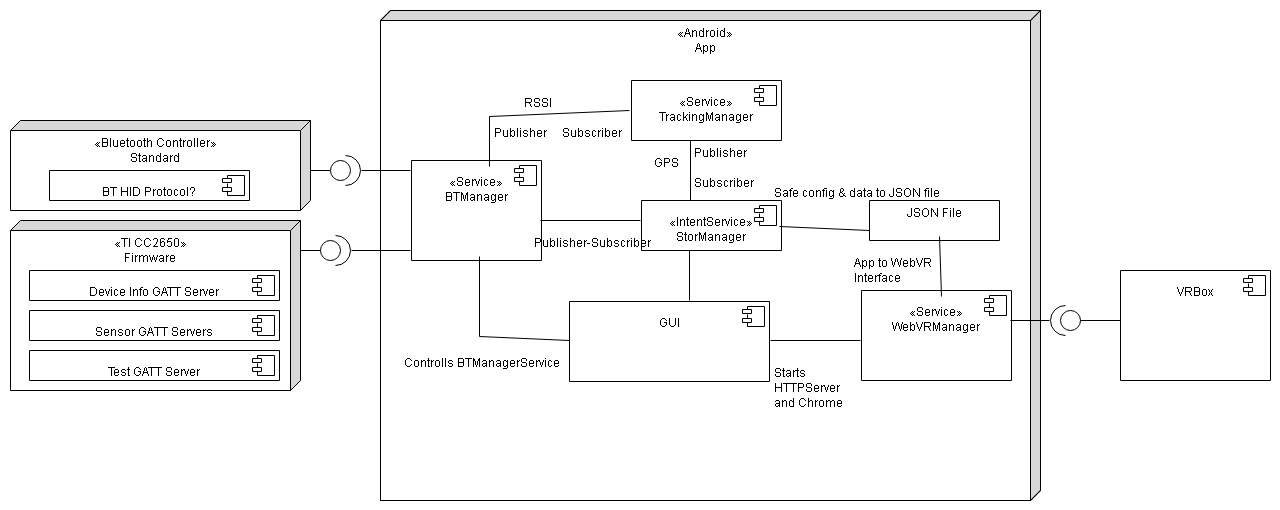
\includegraphics[width=1.4\textwidth]{pics/composite_app.png}


\subsection{Component Decomposition}

\subsubsection{Services}

\begin{itemize}
  \item \textbf{BluetoothManager:} Uses the android.bluetooth and especially the android.bluetooth.le libraries to fetch the sensor data from the sensor device. \\

  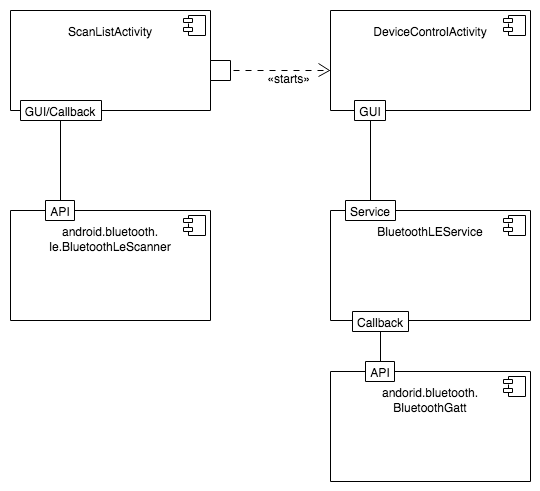
\includegraphics[width=0.8\textwidth]{pics/ble_man.png}
  
  \item \textbf{TrackingManager:} Handles the tracking of the (current) location where the data are recorded. The current position is determined by GPS and enhanced by the cellphone sensor and wifi data.

 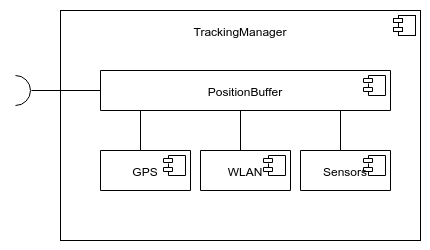
\includegraphics[width=0.8\textwidth]{pics/TrackingManager_Composition.png}

  \item \textbf{StorageManager:} Processes the data provided by the TrackingManager and the BluetoothManager. Uses a JSON file to store data.

 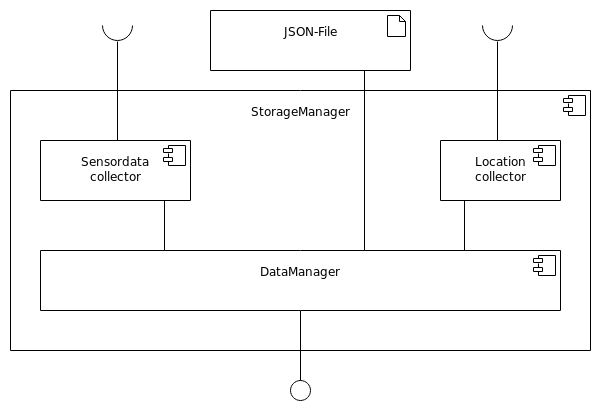
\includegraphics[width=0.8\textwidth]{pics/StorageMgr_Composition.png}

  \item \textbf{WebVRManager:} Handles the display of the virtual reality scene and the given data from the sensor.

 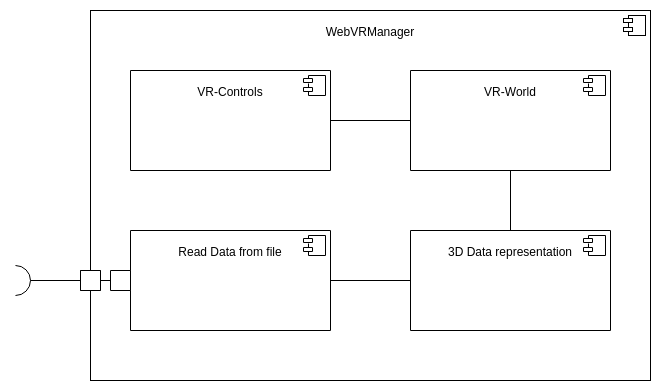
\includegraphics[width=0.8\textwidth]{pics/WebVRManager.png}

\end{itemize}

\subsubsection{GUI}

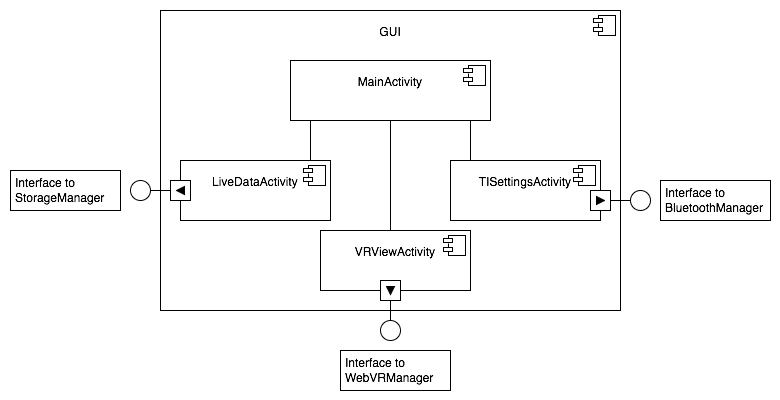
\includegraphics[width=0.8\textwidth]{pics/GUI.png}

\begin{itemize}
  \item \textbf{MainActivity} Provides the main startup screen as the main entry point.
  \item \textbf{VRViewActivity} Shall open a new browser window to display the WebVR webpage.
  \item \textbf{LiveDataActivity} Shall provide a view of the sensor data in human readable form.
  \item \textbf{TISettingsActivity:} Shall provide a settings screen containing scanning and connecting, connected devices and device settings fragments.
  \begin{itemize}
    \item \textbf{ScanningConnectingFragment} shall show the scanning results, delivered by the SensorTagBluetoothReceiverService and provide a connect on/off control.
    \item \textbf{ConnectedDevicesFragment} shall show the connected devices and a short info about the current setting and state of the sensor device.
    \item \textbf{ConnectedDevicesSettingsFragment} shall implement the configuration of the app features of the sensor.
  \end{itemize}
\end{itemize}

\subsubsection{Additional Classes}
\begin{itemize}
  \item \textbf{GATT Profiles} (for each sensor one)
  \item \textbf{GATT Sensor Service UUIDs}
  \item \textbf{Parser Functions} because the BLE protocol implemented in the TI CC2650 delivers raw sensor output
\end{itemize}
 \newpage
  \section{Product Data}

\subsection{VR-World}

\begin{description}
  \item[D1.1] \textbf{Models:} The modeles used to render the VR-World will be saved as .obj files using Blender in /webvr/models/.
  \item[D1.2] \textbf{Textures:} As .png files in /webvr/img/.
\end{description}

\subsection{Bluetooth Functionality}

\begin{description}
 \item[Service UUIDs]
   \begin{description}
     \item[Device Info Service] 0000180a-0000-1000-8000-00805f9b34fb
     \item[Firmware Revision]  00002A26-0000-1000-8000-00805f9b34fb

     \item[IR Temprature Service] f000aa00-0451-4000-b000-000000000000
     \item[IR Temprature Data] f000aa01-0451-4000-b000-000000000000
     \item[IR Temprature Configuration] f000aa02-0451-4000-b000-000000000000
     \item[IR Temprature Time Period] f000aa03-0451-4000-b000-000000000000

     \item[Accelerometer Service] f000aa10-0451-4000-b000-000000000000
     \item[Accelerometer Data] f000aa11-0451-4000-b000-000000000000
     \item[Accelerometer Configuration] f000aa12-0451-4000-b000-000000000000
     \item[Accelerometer Time Period] f000aa13-0451-4000-b000-000000000000

     \item[Humidity  Service] f000aa20-0451-4000-b000-000000000000
     \item[Humidity Data] f000aa21-0451-4000-b000-000000000000
     \item[Humidity Configuration] f000aa22-0451-4000-b000-000000000000
     \item[Humidity Time Period] f000aa23-0451-4000-b000-000000000000

     \item[Magnetometer Service] f000aa30-0451-4000-b000-000000000000
     \item[Magnetometer Data] f000aa31-0451-4000-b000-000000000000
     \item[Magnetometer Configuration] f000aa32-0451-4000-b000-000000000000
     \item[Magnetometer Time Period] f000aa33-0451-4000-b000-000000000000

     \item[Optical  Service] f000aa70-0451-4000-b000-000000000000
     \item[Optical Data] f000aa71-0451-4000-b000-000000000000
     \item[Optical  Configuration] f000aa72-0451-4000-b000-000000000000
     \item[Optical  Time Period] f000aa73-0451-4000-b000-000000000000

     \item[Barometer Service] f000aa40-0451-4000-b000-000000000000
     \item[Barometer Data] f000aa41-0451-4000-b000-000000000000
     \item[Barometer Configuration] f000aa42-0451-4000-b000-000000000000
     \item[Barometer Calibraton] f000aa43-0451-4000-b000-000000000000
     \item[Barometer Time Period] f000aa44-0451-4000-b000-000000000000

     \item[Gyrometer Service] f000aa50-0451-4000-b000-000000000000
     \item[Gyrometer Data] f000aa51-0451-4000-b000-000000000000
     \item[Gyrometer Configuration] f000aa52-0451-4000-b000-000000000000
     \item[Gyrometer Time Period] f000aa53-0451-4000-b000-000000000000

     \item[Movement Service] f000aa80-0451-4000-b000-000000000000
     \item[Movement Data] f000aa81-0451-4000-b000-000000000000
     \item[Movement Configuration] f000aa82-0451-4000-b000-000000000000
     \item[Movement Time Period] f000aa83-0451-4000-b000-000000000000

     \item[Test Service] f000aa64-0451-4000-b000-000000000000
     \item[Test Data] f000aa65-0451-4000-b000-000000000000 shall equal the test result
   \end{description}
   Period in tens of milliseconds
   Configuration: 0: disable, 1: enable; in case of 3D value: 0: disable, bit 0: enable x, bit 1: enable y, bit 2: enable z
\end{description}
 \newpage
 % \input{PH06-ui} \newpage
  \section{Quality Requirements}

%\comment{Auf welche Qualitätsanforderungen (Zuverlässigkeit, Robustheit, Benutzungsfreundlichkeit, Effizienz, ...) wird besonderen Wert gelegt?}

\begin{center}
 \begin{tabular}{lcccc}
  \hline
   & very important & important & less important & lesser important \\
  \hline 
  \multicolumn{5}{l}{\textbf{Functionality}} \\
  
  \quad\textit{Adequacy}&&\textbf{X}&&\\
  \quad\textit{Correctness}&&\textbf{X}&&\\
  \quad\textit{Interoperability}&&&& \textbf{X}\\
  \quad\textit{Security}&&&&\textbf{X}\\
 
  \hline
  \textbf{Reliability}&&\textbf{X}&&\\
 
  \hline
  \multicolumn{5}{l}{\textbf{Usability}}\\
  \quad\textit{Comprehensibleness}&&&\textbf{X}&\\
  \quad\textit{Usability}&&&\textbf{X}&\\
  \hline
  \multicolumn{5}{l}{\textbf{Efficiency}}\\
  \quad\textit{Time response}&&&\textbf{X}&\\
  \quad\textit{Resource costs}&&&\textbf{X}&\\
  \hline
  \textbf{Portability}&&&&\textbf{X}\\
  \hline
  \end{tabular}
\end{center}

\bigskip

\begin{description}
	\item[Functionality] All functions should work as intended, but neither the interaction with other software nor the security of the system is taken into account.
	
	\item[Reliability] Errors should be reduced to a reasonable amount.
	
	\item[Usability] The App should be usable, but user-friendliness is not stressed during the development.
	
	\item[Efficiency] The App should respond in reasonable time to inputs. It also should use reasonable amounts of processor time and storage.
	
	\item[Portability] The App will be developed for Android without consideration for other operating system. 
\end{description}

 \newpage
  \section{Test Cases}

%\comment{Was sind typische Szenarien, die das Produkt erfüllen muss?}
%\comment{tests für alle requirements; am ende}

%Jede Produktfunktion \textit{/F????/} wird anhand von konkreten Testfällen \textit{/T????/} getestet.\\
%Die dabei verwendeten Namen werden rein zufällig gewählt.

%\begin{description}
%  \item[/T????/]
%    ...
%\end{description}


\begin{description}
  \item[/T0300/]
    \textit{Look around:} While in normal 3D mode the tester shall click the screen and drag first up to move the camera up.
    Then move down to move the camera down, then at last left and then right, all the time the camera must follow the movement of the finger.
    After this the tester shall tilt the phone up to move the camera up, then tilt it down, left and right. The camera shall follow the tilt direction of the phone all the time with no delay.

    This test shall be repeated in stereoscopic 3D view. While the clicking and dragging shall not work, the tilting of the phone shall be the only way to pan the camera.
\end{description}

\begin{description}
  \item[/T0310/]
    \textit{Move inside the virtual reality scene:} While in normal 3D mode the tester shall tilt the joystick on the controller forward and the camera shall move forward.
    By tilting the joystick backward the camera shall move back, by tilting left the camera shall move left and by tilting right it shall move right.
    The camera shall allways follow the view point, so forward is allways in the center of the camera.

    This test shall be again repeated in stereoscopic 3D view and all functions shall work the same.
\end{description}

\begin{description}
	\item[/T0320/]
	\textit{Searching, connecting and disconnecting devices:} The tester shall search a sensor device by pressing the "scan" button in the settings menu. All devices nearby shall be shown in a list with distinguishable entries. By tapping on a list entry a connection to the device shall be established.
	By tapping again on the list entry the connection shall be terminated.
\end{description}

\begin{description}
	\item[/T0330/]
	\textit{Displaying temperature:} While in normal 3D mode and with a established connection to a sensor device the tester shall look around. At the position of the device a glowing sphere shall be displayed.
	
	This test shall be again repeated in stereoscopic 3D view and shall work the same.
\end{description}

\begin{description}
	\item[/T0340/]
	\textit{Trensferring Bluetooth data:} When the connection to a sensor device is established, the tester shall enter the data view wihin the app and see some representation of the transmitted data which allows him to check the connectivity and functionality to/ of the sensor device.
\end{description} \newpage
%  \section{Development Environment}

\subsection{Software}

\begin{itemize}
  \item[OS] Windows 10, macOS Sierra, Linux Mint 18.1
  \item[IDEs]  Android Studio, Sensor Controller Studio 1.4.1, Atom, Chrome DevTools
  \item[VCS] Git, GitHub
  \item[UML-Editor] Enterprise Architekt, MS Visio, \href{draw.io}{draw.io}, UMLetino
  \item[Zeichensatz] \LaTeX

\end{itemize}

\subsection{Hardware}

\begin{itemize}
  \item[Smartphone] Motorola XT1572
  \item[Sensor] TI CC2650STK
  \item[VR-Headset] Victorstar VRBox 2.0
  \item[Bluetooth-Controller] VR-Park distributed with VRBox 2.0
\end{itemize}
 \newpage
  \section{Project Time Line}


\begin{tabular}{l|p{12cm}}

\textbf{Week / Final Date}  & \textbf{Event / Tasks} \\ \hline

\textbf{25.5.- 1.5.} & first research, write Software Specification \\ 
2.5. & release SW Specification, project plan, subjects of milestones\\ \hline
\textbf{2.5.- 8.5.} & distribute tasks, decide on design\\ 
\textbf{9.5.- 15.5.} & start building, finalize SW Spezification \\ 
\textbf{16.5.- 22.5.} & \\
22.5. & \textit{Milestone 1:} Bluetooth and sensor location data can be gathered, a VR-Room is built, a GUI is implemented\\ \hline
\textbf{23.5.- 29.5.} &  \\
\textbf{30.5.- 5.6.} & \\
\textbf{6.6.- 12.6.} & \\
12.6. & \textit{Milestone 2:} Gathered data can be displayed in 3D, \textit{intermediate assessment} \\ \hline
\textbf{13.6.- 19.6.} & \\
\textbf{20.6.- 26.6.} & \\
\textbf{27.6.- 3.7.} & \\
\textbf{4.7.- 10.7.} & \\
\textbf{11.7.- 17.7.} & \\
17.7. & \textit{Milestone 3:} All functionalities are implemented and successfully tested. \\ \hline
\textbf{18.7.- 24.7.} & prepare presentation and usage examples\\
25.7. & \textit{final presentation }

\end{tabular} \\



%Possible starting points: \\
%\href{https://bitbucket.org/StylingAndroid/bluetoothle/src/1fe191cf34f34f9917b1d0d62c617c607fe3df4d/src/main/java/com/stylingandroid/ble/?at=Part2}{Simple, bad layout} \\
%\href{https://git.ti.com/sensortag-20-android/sensortag-20-android/trees/master/sensortag20/BleSensorTag/src/main/java/com/example/ti}{TI official, complex}
 \newpage
 % \section{Abbreviations}

\begin{tabular}{rl}
TI & Texas Instruments\\
VR & Virtual Reality\\
DB & Database\\
App & Application\\
BLE & Bluetooth Low Energy\\

\end{tabular}
\bigskip

\section{Glossary}

\begin{tabular}{r p{11cm}}
Bluetooth & Technology for wireless transmitting data between devices in close proximity.\\
Bluetooth Low Energy & More energy efficient version of Bluetooth.\\
TI SimpleLink SensorTag & Device that provides data from multiple sensors via a Bluetooth interface.\\
Virtual Reality & Visual 3D computer simulation of a real world.\\
Stereoscopic 3D & The impression of 3D is created by rendering different pictures for every eye of the viewer.\\
Augmented Reality & A view of the real world gets combined with images from the VR-World.\\
Gyroscope sensor & Sensor for measuring orientation in space.\\
\end{tabular} \newpage
\end{document}
